 %%
%%
\documentclass[12pt]{book}
\usepackage{amsfonts}
\usepackage{amsmath}
\usepackage{amssymb}
\usepackage{graphicx}
\usepackage{hyperref}
\usepackage{float}
\usepackage{xcolor}
\usepackage{tabularx}
\setlength{\textheight}{10in}
\setlength{\textwidth}{7.4in}
\setlength{\topmargin}{-0.75in}
\setlength{\oddsidemargin}{-0.5in}
\setlength{\evensidemargin}{-0.5in}
\setlength{\parskip}{0.15in}
\setlength{\parindent}{0in}

\begin{document}


\vspace{-1.0in}\begin{center}
\Large{MHF4UR : Pre-AP Advanced Functions }

\Large{Assignment \#3}


\end{center}

%\medskip

\vspace{0.015in}\hrulefill\ 

\textbf{Reference Declaration} %  Fill in your Reference Declarations in this section before your submit your assignment.

Complete the Reference Declaration section below in order for your assigment to be graded.

If you used any references beyond the course text and lectures (such as other texts, discussions with colleagues or online resources), indicate this information in the space below.  If you did not use any aids, state this in the space provided. 

Be sure to cite appropriate theorems throughout your work. You may use shorthand for well-known theorems like the FT (Factor Theorem), RRT (Rational Root Theorem), etc. 

Note: Your submitted work must be \textbf{your original work}. 

Family Name: Do\\%Family Name Here
First Name: Kien%First Name Here

Declared References:\\
Read more on radians and took images from this website:\\
https://mathbitsnotebook.com/Algebra2/TrigConcepts/TCRadianMeasure.html\\

Asked my dad for help with question 8 and question 10(b).\\
For question 10(b), I learned the formula to determine the sum of n odd numbers from here:\\https://www.quora.com/What-is-the-formula-for-the-sum-of-n-odd-numbers

% Type your references here.
% You can use as many lines as required.

\vspace{0.015in}\hrulefill\ 

\newpage

%%%%%%%%%%%% PROBLEMS START HERE

\begin{enumerate}

%% PROBLEM 1
\item Demonstrate that $\sin^2(x) + \cos(x) = \cos^2(x) + \sin(x)$ is not an identity by means of a counterexample.\\


\textbf{Solution:}\\
Sub in $x = \dfrac{\pi}{6}$. If this value of $x$ does not yield the same value on the both sides of the equation, I will have successfully demonstrated that $\sin^2(x) + \cos(x) = \cos^2(x) + \sin(x)$ is not an identity by means of counterexample.\\
\begingroup
\addtolength{\jot}{0.5em}
\begin{align*}
    \sin^2(x) + \cos(x) &= \cos^2(x) + \sin(x)\xleftarrow[]{\textbf{sub in $\dfrac{\pi}{6}$}}\\ %%endl
    \sin^2\left(\dfrac{\pi}{6}\right) + \cos\left(\dfrac{\pi}{6}\right) &= \cos^2\left(\dfrac{\pi}{6}\right) + \sin\left(\dfrac{\pi}{6}\right)\\ %% endl
    \left(\dfrac{1}{2}\right)^2 + \left(\dfrac{\sqrt{3}}{2}\right) &= \left(\dfrac{\sqrt{3}}{2}\right)^2 + \left(\dfrac{1}{2}\right)\\ %% endl
    \dfrac{1}{4} + \dfrac{\sqrt{3}}{2} &= \dfrac{3}{4} + \dfrac{1}{2}\\ % endl
    \dfrac{1 + 2\sqrt{3}}{4} &= \dfrac{3+2}{4}\\
    1+2\sqrt{3} &= 5\\
    2\sqrt{3} &= 4
\end{align*}
\endgroup
We can see that for the left side to equal the right side, the left side needs to be $2\times2$, or, $2\times \sqrt{4}$. Since $\sqrt{3} < \sqrt{4}$, the left side yields a value lower than the right side. For an expression to be an identity, both sides must be equal to each other for all values of $x$. Since $2\sqrt{3} \neq 4$, the left side does not equal the right side. This means $\sin^2(x) + \cos(x) = \cos^2(x) + \sin(x)$ is not an identity.\\

\textbf{Therefore, $\sin^2(x) + \cos(x) = \cos^2(x) + \sin(x)$ is not an identity.}

\vspace{0.3cm}

\newpage

%% PROBLEM 2
\item Prove the identity $\sin(x)\cos(x)=1-\dfrac{\sin^2(x)}{1+\cot(x)}-\dfrac{\cos^2(x)}{1+\tan(x)}$. Remember to use proper form for proving trigonometric identities by indicating the identities you are using.\\

\textbf{Solution:}\\
Manipulate the right side to equal the left side.
\begingroup
\addtolength{\jot}{0.5em}
\begin{align*}
    1-\dfrac{\sin^2(x)}{1+\cot(x)}-\dfrac{\cos^2(x)}{1+\tan(x)} &= 1- \dfrac{\sin^2(x)}{1 + \dfrac{\cos(x)}{\sin(x)}} - \dfrac{\cos^2(x)}{1 + \dfrac{\sin(x)}{\cos(x)}}  \xleftarrow{\textbf{Quotient identity}} \\%%endl
    &= 1- \dfrac{\sin^2(x)}{\dfrac{\sin(x)}{\sin(x)} + \dfrac{\cos(x)}{\sin(x)}} - \dfrac{\cos^2(x)}{\dfrac{\cos(x)}{\cos(x)} + \dfrac{\sin(x)}{\cos(x)}} \\%%endl
    &= 1- \dfrac{\sin^2(x)}{\dfrac{\sin(x) + \cos(x)}{\sin(x)}} - \dfrac{\cos^2(x)}{\dfrac{\cos(x) + \sin}{\cos(x)}} \\%%endl
    &= 1- \dfrac{\sin^3(x)}{\sin(x)+\cos(x)} - \dfrac{\cos^3(x)}{\sin(x)+\cos(x)}\\%%endl
    &= 1+ \left(-\dfrac{\sin^3(x)}{\sin(x)+\cos(x)} -  \dfrac{\cos^3(x)}{\sin(x)+\cos(x)}\right)\\%%endl
    &= 1- \left(\dfrac{\sin^3(x)}{\sin(x)+\cos(x)} + \dfrac{\cos^3(x)}{\sin(x)+\cos(x)}\right)\\%%endl
    &= 1- \left(\dfrac{\sin^3(x) + \cos^3(x)}{\sin(x)+\cos(x)}\right)\xleftarrow[a^3+b^3 = (a+b)(a^2-ab+b^2)]{\textbf{Polynomial identity}}\\%%endl
    &= 1- \dfrac{(\sin(x)+\cos(x))(\sin^2(x)-\sin(x)\cos(x)+\cos^2(x))}{\sin(x)+\cos(x)} \\%%endl
    &= 1-(\sin^2(x)-\sin(x)\cos(x)+\cos^2(x)) \xleftarrow[\sin^2(x) + \cos^2(x) = 1]{\textbf{Pythagorean identity}}\\ %%endl
    &= 1-(1-\sin(x)\cos(x)) \\ %%endl
    &= \sin(x)\cos(x)
\end{align*}
\endgroup
\textbf{Therefore, $\sin(x)\cos(x)=1-\dfrac{\sin^2(x)}{1+\cot(x)}-\dfrac{\cos^2(x)}{1+\tan(x)}$ is an identity.}

\newpage

%% PROBLEM 3
\item Determine equivalent expressions for both of $\sin(4x)$ and $\cos(4x)$ entirely in terms of $x$. You do not need to justify your steps.\\

\textbf{Solution:}\\
Determine the equivalent expression for $\sin(4x)$.
\begin{align*}
    \sin(4x) &= 2 \sin (2x) \cos(2x)\\
    \sin(4x) &= 2\left[2\sin\left(x\right)\cos\left(x\right)\right]\left[1-2\sin^{2}\left(x\right)\right]\\
    \sin(4x) &= 4\left[\sin\left(x\right)\cos\left(x\right)\right]\left[1-2\sin^{2}\left(x\right)\right]
\end{align*}
Determine the equivalent expression for $\cos(4x)$.
\begin{align*}
    \cos(4x) &= 1-2\sin^{2}\left(2x\right) \\
    \cos(4x) &= 1-2\left(\sin\left(2x\right)\sin\left(2x\right)\right) \\
    \cos(4x) &= 1-2\left(2\sin\left(x\right)\cos\left(x\right)\cdot2\sin\left(x\right)\cos\left(x\right)\right) \\
    \cos(4x) &= 1-2\left(4\sin^{2}\left(x\right)\cos^{2}\left(x\right)\right) \\
    \cos(4x) &= 1-8\sin^{2}\left(x\right)\cos^{2}\left(x\right)
\end{align*}

\textbf{Therefore, the equivalent expression for $\sin(4x)$ is $4\left[\sin\left(x\right)\cos\left(x\right)\right]\left[1-2\sin^{2}\left(x\right)\right]$ and the equivalent expression for $\cos(4x)$ is $1-8\sin^{2}\left(x\right)\cos^{2}\left(x\right)$.}

\newpage

%% PROBLEM 4
\item A circle is centered at the origin with a radius of 25. Inside this circle is an inscribed rectangle with its bottom edge on the x-axis and the two vertices on the opposite side on the circumference of the circle,. Represent the area, $A$, of the rectangle:

\begin{enumerate}
\item In terms of $x$, the distance between the y-axis and the right leg of the rectangle. \\

\textbf{Solution:}\\
Let the length of the x-axis be $x$ and the length of the y-axis be $y$.\\

Determine the length of $y$ given $x$ using the Pythagorean theorem.
\begin{align*}
    x^2 + y^2 &= 25^2 \\
    y^2 &= 25^2 - x^2 \\
    y &= +\sqrt{625 - x^2} \xleftarrow[\textbf{lengths cannot be negative}]{\textbf{only take positive values}}
\end{align*}
Since we now know what $y$ equals. We can determine the area of the rectangle in quadrant 1. However, the exact same rectangle is also in quadrant 2 so we must double the area of the rectangle in quadrant 1. This means the area, $A$ can be represented as
$$A = 2x(\sqrt{625-x^2})$$

\textbf{Therefore, the area of the rectangle in terms of $x$ is $A = 2x(\sqrt{625-x^2})$.}\\

\item In terms of $\theta$, where $\theta$ is an angle in standard position with its terminal arm on the upper right vertex of the rectangle.\\

\textbf{Solution:}\\
Since the terminal arm of the angle $\theta$ can only be in quadrant 1, we can assume that $0 \leq \theta \leq \dfrac{\pi}{2}$.\\

To determine the area, we need to know the side lengths. Since we know the radius and are determining the area in terms of $\theta$, we can use trigonometric ratios to determine side lengths $x$ and $y$ which will allow us to determine the area of the rectangle. In this case, the radius is the hypotenuse, side $x$ is the adjacent side to $\theta$ and side $y$ is opposite to $\theta$.\\

Determine an expression for side $x$. 
\begingroup
\addtolength{\jot}{0.3em}
\begin{align*}
    \cos\theta &= \dfrac{x}{25}\\
    x &= 25\cos\theta
\end{align*}
\endgroup
Determine an expression for side $y$. 
\begingroup
\addtolength{\jot}{0.3em}
\begin{align*}
    \sin\theta &= \dfrac{y}{25}\\
    y &= 25\sin\theta
\end{align*}
\endgroup
Now that we have an expression for side $x$ and side $y$, we can determine the area of the rectangle by substituting the expressions into $2(x \times y)$. This means, $A$ can be represented as
$$A = 2(25\cos\theta)(25\sin\theta)$$
$$A = 1250\cos(\theta)\sin(\theta)$$
\textbf{Therefore, the area of the rectangle in terms of $\theta$ is $A = 1250\cos(\theta)\sin(\theta)$}.
\end{enumerate}

\newpage


%% PROBLEM 5
\item Create a one-page summary of information about radian measure that reflects your understanding of trigonometric functions. You should include graphic(s) where it is useful to do so.\\

\textbf{Explanation:}\\
\begin{minipage}{.5\textwidth}
The radian is a measurement that represents the size of an angle. Rather than directly expressing the size of an angle using degrees, the radian is expressed in terms of the length of an arc, \textcolor{red}{s}, that subtends the angle, $\theta$, at  the centre of a circle with radius \textcolor{red}{r}.\\
\end{minipage}
\begin{minipage}{0.5\textwidth}
    \begin{figure}[H]
    \centering{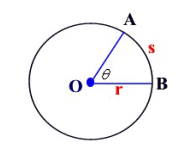
\includegraphics[width=4cm]{Q5_1.png}}
    \end{figure} 
\end{minipage}
The unit of measure, radian, is proportional to \textcolor{red}{r} and $\theta$, and is equal to $\dfrac{s}{r}$. In other words, it is a measurement of the distance along the unit circle. Since both the arc length and the radius are measured in units of length, the result is a real number without any units.\\
%%========================
\begin{minipage}{.5\textwidth}
    If the length of an arc of a circle, \textcolor{red}{s} is the same as the length of the circle's radius, \textcolor{red}{r}, a specific situation occurs. The angle, $\theta$, created by this situation is \textbf{one radian}.
    
    $$\theta = \dfrac{s}{r} = \dfrac{r}{r} = 1$$
\end{minipage}
\begin{minipage}{.5\textwidth}
    \begin{figure}[H]
    \centering{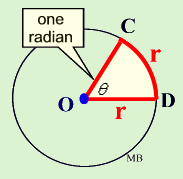
\includegraphics[width=4cm]{Q5_2.png}}
    \end{figure} 
\end{minipage}\\

\textbf{Converting from radians to degrees and vice versa}\\
\begin{minipage}{.5\textwidth}
    Consider the arc length created by an angle of $360^{\circ}$. We know this arc length is $2\pi r$, the formula used to determine the circumference of a circle. Using the relationship $\dfrac{s}{r}$, the size of the angle can be expressed in radians.
    $$\theta = \dfrac{2\pi r}{r} = 2\pi \enskip \text{radians}$$
\end{minipage}
\begin{minipage}{.5\textwidth}
    \begin{figure}[H]
    \centering{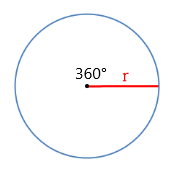
\includegraphics[width=4cm]{Q5_3.png}}
    \end{figure} 
\end{minipage}\\
Since $\theta = 2\pi \enskip \text{radians}$ and $\theta = 360^{\circ}$, we can say that $$2\pi \enskip \text{radians} = 360^{\circ}$$
$$\pi \enskip \text{radians} = 180^{\circ}$$
%%Knowing this, we can determine what 1 radian is in degrees.
%%$$\dfrac{\pi \enskip \text{radians}}{\pi} = \dfrac{180^{\circ}}{\pi}$$
%%$$1 \enskip \text{radian} \approx 57.3^{\circ}$$
For converting degrees to radians and vice versa, we can multiply by 1, or, $\dfrac{180^{\circ}}{\pi}$, $\dfrac{\pi}{180^{\circ}}$ to get an equivalent expression.\\
\textbf{Example: Convert $20^{\circ}$ to radians}
\begin{align*}
    20^{\circ} &= 20^{\circ} \times 1 \\
    &= 20^{\circ} \times \dfrac{\pi}{180^{\circ}} \xleftarrow[\text{have } 180^{\circ} \text{ be in the denominator}]{\text{to divide out the degrees}} \\
    &= \dfrac{\pi}{9} \xleftarrow[]{\text{exact final answer}} \\
    &\approx 0.35
\end{align*}
Therefore, $20^{\circ} \approx 0.35 \enskip \text{radians}$.
\newpage

%% PROBLEM 6
\item Solve $2\sin^2(x) + \sin(2x) = 2$ $(x \in \mathbb{R})$. Be sure to effectively communicate the multiple solutions.\\

\textbf{Solution:}\\
Simplify this equation.
\begin{align*}
    2\sin^2(x) + \sin(2x) &= 2\\
    2\sin^2(x) + 2\sin(x)\cos(x) &= 2\\
    2(\sin^2(x) + \sin(x)\cos(x) &= 2\\
    2(\sin^2(x) + \sin(x)\cos(x) &= 2\\
    \sin^2(x) + \sin(x)\cos(x) &= 1\\
    \sin^2(x) - \sin^2(x) + \sin(x)\cos(x) &= 1 - \sin^2(x)\\
    \sin(x)\cos(x) &= \cos^2(x) \\
    \sin(x)\cos(x) - \cos^2(x) &= 0 \\
    \cos(x) \times (\sin(x) - \cos(x)) &= 0 \xleftarrow[(\sin(x) - \cos(x)) = 0 \text{ is true iff } \sin(x) = \cos(x)]{\text{true if } \cos(x) = 0 \text{ or } (\sin(x) - \cos(x)) = 0}
\end{align*}
\begin{minipage}{.5\textwidth}
    \begin{align*}
        &\textbf{Case 1:}\\
        &\cos(x) = 0 \text{ iff } x = \dfrac{\pi}{2} + k\pi \quad \{k \in \mathbb{Z}\}
    \end{align*}
\end{minipage}
\begin{minipage}{.5\textwidth}
    \begin{align*}
        &\textbf{Case 2:}\\
        &\sin(x) - \cos(x) = 0 \text{ iff } x = \dfrac{\pi}{4} + k\pi \quad \{k \in \mathbb{Z}\}
    \end{align*}
\end{minipage}\\

\textbf{Therefore, $x = \dfrac{\pi}{2} + k\pi$ or $x = \dfrac{\pi}{4} + k\pi \quad \{k \in \mathbb{Z}\}$}


\newpage

%% PROBLEM 7
%\begin{minipage}{4in}
\item Go to the website of the \href{http://worldweather.wmo.int/}{World Meteorological Organization} and select a city from the map (right).
Once you select a city, click on Climatological Information which is a tab above the map. Locate and record the data for mean max. temperature and mean min. temperature into a table. Using the data, create models for the relationship between the day of the year and both the high and low mean respectively. Finally, test the accuracy of each model by using it to determine the temperature for a single day, each.\\\\
%\end{minipage}\hspace{0.2in}
%%\begin{minipage}{1in}
%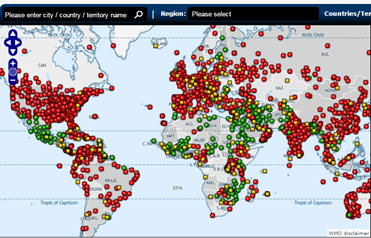
\includegraphics[scale=0.75]{WorldMap.png}
%\end{minipage}\\
\textbf{Solution:}\\
Step 1: Record the data for mean max. temp. and mean min. temp. of Toronto into a table.
\begin{center}
\textbf{Mean Daily Minimum and Maximum Temperature for the city of Toronto}
\end{center}
\begin{tabularx}{0.8\textwidth} { 
  | >{\raggedright\arraybackslash}X 
  | >{\centering\arraybackslash}X 
  | >{\raggedleft\arraybackslash}X | }
 \hline
 Month & Mean Daily Minimum Temperature ($^{\circ}$C) & Mean Daily Maximum Temperature ($^{\circ}$C) \\
 \hline %jan
 Jan  & -7.3  & -1.1  \\
 \hline %feb
 Feb  & -6.3  & -0.2  \\
 \hline %mar
 Mar  & -2.0  & 4.6  \\
 \hline %apr
 Apr  & 3.8  & 11.3  \\
 \hline %may
 May  & 9.9  & 18.5  \\
 \hline %jun
 Jun  & 14.8  & 23.5  \\
 \hline %jul
 Jul  & 17.9  & 26.4  \\
 \hline %aug
 Aug  & 17.3  & 25.3  \\
 \hline %sep
 Sep  & 13.2  & 20.7  \\
 \hline %oct
 Oct  & 7.3  & 13.8  \\
 \hline %nov
 Nov  & 2.2  & 7.4  \\
 \hline %dec
 Dec  & -3.7  & 1.8  \\
\hline %% keep this at the end
\end{tabularx}\\

Step 2: Create a model for the relationship between the month of the year and the minimum temperature / maximum temperature. I will display the finished graph then explain how I applied the transformations to get that final graph.\\

a) Month vs. Mean Daily Minimum Temperature \\
\begin{figure}[H]
\centering{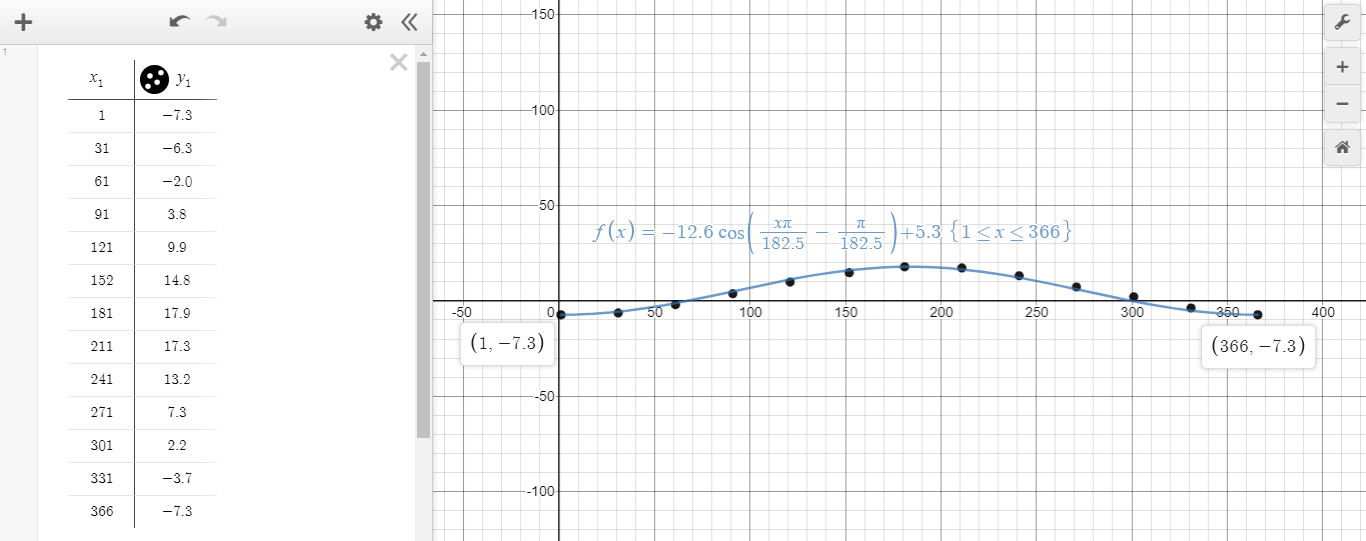
\includegraphics[width=19cm]{Q7_1.png}}
\end{figure}
The figure above represents the Mean Daily Minimum Temperature of Toronto over a course of 365 days. The function is $f\left(x\right)=-12.6\cos\left(\dfrac{x\ \pi}{182.5}-\dfrac{\pi}{182.5}\right)+5.3\left\{1\le x\le366\right\}$. The domain is restricted from 1 to 366, inclusive. It is assumed that each month has 30 days and that January starts at 1 on the $x$-axis. That means February would start on day 31, March on day 61, etc. Since the model is an estimate, December will have 5 extra days to make the year have 365 days. 
\begin{itemize} %% begin itemize =============================
  \item \textbf{Parent function cos:} $\cos$ either starts at the highest or the lowest point in a sinusoidal function. Since the temperature was lowest in January out of all the months, $\cos$ was chosen as the parent function instead of $\sin$.\\
  $\therefore$ We have: $f(x) = \cos(x) \left\{1\le x\le 366\right\}$
  
  \item \textbf{Vertical stretch factor 12.6:} The vertical stretch and compression is determined by the coefficient of $\cos$, or, the amplitude. This was determined by taking the coordinate of the highest value on the y-axis subtract the coordinate of the lowest value on the y-axis, then the result is divided by 2. The highest temperature is 17.9 and the lowest temperature is -7.3. Therefore, we have $\dfrac{17.9 - (-7.3)}{2} = 12.6$.\\
  $\therefore$ We have: $f(x) = 12.6\cos(x) \left\{1\le x\le 366\right\}$
  
  \item \textbf{Reflection on the x-axis:} The temperature continues to rise starting at January so the coefficient of cos is $-12.6$.\\
  $\therefore$ We have: $f(x) = -12.6\cos(x) \left\{1\le x\le 366\right\}$
  
  \item \textbf{Horizontal stretch of $\dfrac{\pi}{182.5}$:} The coefficient of $x$ in $\cos(x)$ is 1 and it has a period of $2\pi$. We know that the period of the graph is 365. To determine the coefficient of $x$ such that the period is $365$, I can take $2\pi$, the non-transformed period, divide it by $365$, the transformed period, to get the desired coefficient of $x$. $\dfrac{2\pi}{365} = \dfrac{\pi}{182.5}$.\\
  $\therefore$ We have: $f\left(x\right)=-12.6\cos\left(\dfrac{x\ \pi}{182.5}\right) \left\{1\le x\le 366\right\}$
  
  \item \textbf{Vertical translation 5.3 units up:} Determining the vertical translation is the same as determining the axis of the sine function. To determine the vertical axis, I take the sum of the highest point and the lowest point and divide it by 2. Therefore, we have $\dfrac{17.9+(-7.3)}{2} = 5.3$.\\
  $\therefore$ We have $f\left(x\right)=-12.6\cos\left(\dfrac{x \pi}{182.5}\right)+5.3 \left\{1\le x\le 366\right\}$
  
  \item \textbf{Horizontal translation $\dfrac{\pi}{182.5}$ right:} Without the translation, the lowest temperature on the graph would be at 0 and 365. Since January is at 1, I need to shift the function right until the lowest temperature corresponds to $x = 1$ on the graph. This means I need to determine the horizontal translation when $x = 1$, $f(x) = -7.3$.\\
  Let $m$ be the horizontal translation. Determine $m$ when $x = 1$, $f(x) = -7.3$ in the function $f\left(x\right)=-12.6\cos\left(\dfrac{x\pi}{182.5} - m\right)+5.3$
  \begin{align*}
      -7.3 &= -12.6\cos\left(\dfrac{\pi}{182.5} - m\right) + 5.3\\
      \cos^{-1}\left(\dfrac{-7.3 - 5.3}{-12.6}\right) &= \dfrac{\pi}{182.5} - m\\
      0 &= \dfrac{\pi}{182.5} - m\\
      m &= \dfrac{\pi}{182.5}
  \end{align*}
  $\therefore$ We have: $f\left(x\right)=-12.6\cos\left(\dfrac{x\ \pi}{182.5}-\dfrac{\pi}{182.5}\right)+5.3\left\{1\le x\le366\right\}$
\end{itemize} %% end itemize =============================
%% ======================= begin 7b ===========================
b) Month vs. Mean Daily Maximum Temperature \\
\begin{figure}[H]
\centering{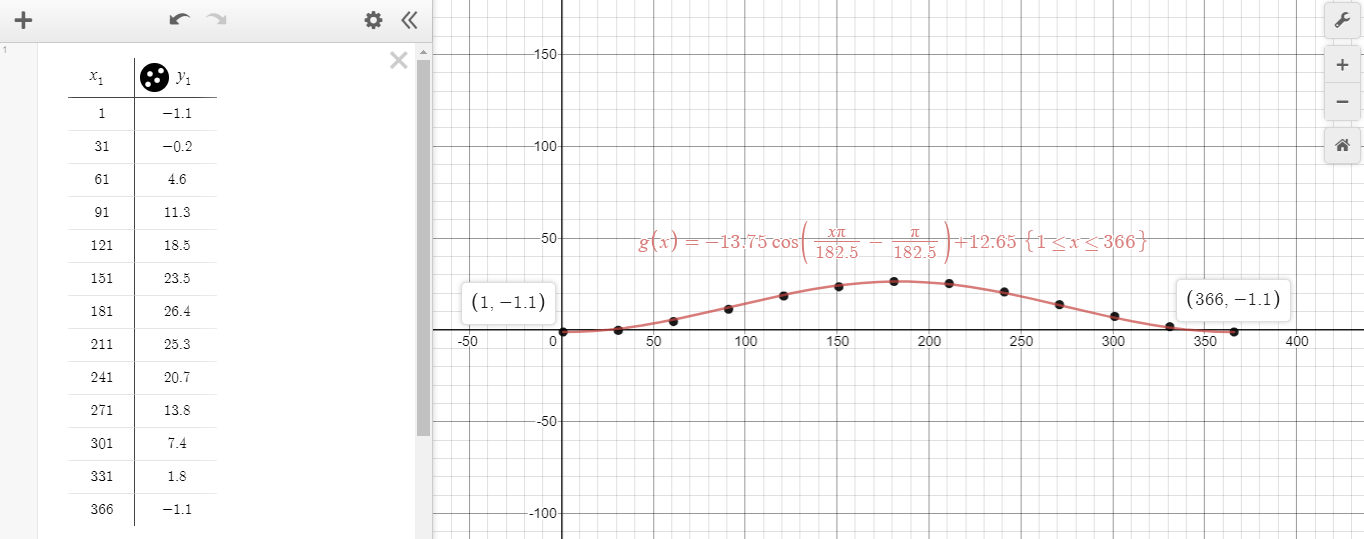
\includegraphics[width=19cm]{Q7_2.png}}
\end{figure}
The figure above represents the Mean Daily Maximum Temperature of Toronto over a course of 365 days. The function is $g\left(x\right)=-13.75\cos\left(\dfrac{x\pi}{182.5}-\dfrac{\pi}{182.5}\right)+12.65\ \left\{1\le x\le366\right\}$. The domain is restricted from 1 to 365, inclusive. It is assumed that each month has 30 days and that January starts at 1 on the $x$-axis and December has 35 days.
\begin{itemize} %% begin itemize =============================
  \item \textbf{Parent function cos:} $\cos$ either starts at the highest or the lowest point in a sinusoidal function. Since the temperature was lowest in January out of all the months, $\cos$ was chosen as the parent function instead of $\sin$.\\
  $\therefore$ We have: $g(x) = \cos(x) \left\{1\le x\le366\right\}$
  
  \item \textbf{Vertical stretch factor 13.75 and vertical reflection:} The highest temperature is 26.4 and the lowest temperature is -1.1. Therefore, we have $\dfrac{26.4 - (-1.1))}{2} = 13.75$. However, the temperature continues to rise starting at January so the coefficient of cos is $-13.75$.\\
  $\therefore$ We have: $g(x) = -13.75\cos(x) \left\{1\le x\le366\right\}$
  
  \item \textbf{Horizontal stretch of $\dfrac{\pi}{182.5}$:} To determine the coefficient of $x$ such that the period is $365$, I can take $2\pi$, the non-transformed period, divide it by $365$, the transformed period, to get the desired coefficient of $x$. $\dfrac{2\pi}{12} = \dfrac{\pi}{365}$.\\
  $\therefore$ We have: $g\left(x\right)=-13.75\cos\left(\dfrac{x\ \pi}{182.5}\right) \left\{1\le x\le366\right\}$
  
  \item \textbf{Vertical translation 5.3 units up:} To determine the vertical axis, I can take the sum of the highest point and the lowest point and divide it by 2. Therefore, we have $\dfrac{26.4+(-1.1)}{2} = 5.3$.\\
  $\therefore$ We have $g\left(x\right)=-13.75\cos\left(\dfrac{x\ \pi}{182.5}\right)+5.3 \left\{1\le x\le366\right\}$
  \newpage %%==================  new page   ================
  \item \textbf{Horizontal translation $\dfrac{\pi}{182.5}$ right:} The horizontal translation of this function is the same as the Mean Minimum Daily Temperature's function. That is because both graphs have a period of 365 with a domain from 1 to 365, inclusive.\\\\
  $\therefore$ We have: $g\left(x\right)=-13.75\cos\left(\dfrac{x\pi}{182.5}-\dfrac{\pi}{182.5}\right)+12.65\ \left\{1\le x\le366\right\}$
\end{itemize} %% end itemize =============================

Step 3: Test the accuracy of each model by using it to determine the temperature for one single day, each. I will test the temperature on day February 14 for both models. Since the corresponding value of $x$ that is equivalent to February 14, let $x = 44$.\\
\begingroup
\addtolength{\jot}{0.8em}
\begin{minipage}{.5\textwidth}
    \begin{align*}
    &\textbf{Daily Min Temp}\\
        f(x)&=-12.6\cos\left(\dfrac{x\pi}{182.5}-\dfrac{\pi}{182.5}\right)+5.3\\
        &= -12.6\cos\left(\dfrac{44\pi}{182.5}-\dfrac{\pi}{182.5}\right)+5.3\\
        &= -12.6\cos\left(\dfrac{43\pi}{182.5}\right)+5.3 \\
        &= -12.6\left(0.7383\right)+5.3 \\
        &= -4.0029 \\
    \end{align*}      
    \end{minipage}
    \begin{minipage}{.5\textwidth}
    \begin{align*}
    &\textbf{Daily Max Temp}\\
        g(x)&=-13.75\cos\left(\dfrac{x\pi}{182.5}-\dfrac{\pi}{182.5}\right)+12.65 \\
        &= -13.75\cos\left(\dfrac{44\pi}{182.5}-\dfrac{\pi}{182.5}\right)+12.65 \\
        &= -13.75\cos\left(\dfrac{43\pi}{182.5}\right)+12.65 \\
        &= -13.75\left(0.7383\right)+12.65 \\
        &= 2.49\\
    \end{align*}
\end{minipage}
\endgroup
The minimum temperature on February 14th is $-4^{\circ}$C and the maximum temperature on February 14th is $-2.49^{\circ}$C.

\newpage

%% PROBLEM 8
\item Given $a,b \in \mathbb{Z}^+$, with $\gcd(a,b)=1$, if $f(x)=\sin(ax)$ and $g(x)=\cos(bx)$ then determine the period of $h(x)=f(x)+g(x)$. Briefly explain and illustrate your methods of determining the period of $h(x)$ and be specific. If your method is through investigation, be certain to cite specific examples, observations and generalizations you are making and explain why they are logical. \\

\vspace{0.2cm}
Recall: The greatest common divisor of two non-zero integers $a$ and $b$ is the greatest integer that divides both $a$ and $b$ and is denoted by $\gcd(a,b)$. If the $\gcd(a,b)=1$ then we say that $a$ and $b$ are \emph{relatively prime} or \emph{coprime}.\\

\textbf{Solution:}\\
Taking a look at $h(x)$, we can see that since $h(x)$ is the sum of $f(x)$ and $g(x)$, the period of $h(x)$ will equal to the distance from the point where $f(x)$ and $g(x)$ intersect to the next point where the intersection looks exactly the same as the previous one.
Or, the period of $h(x)$ can be described as the shortest distance where \textbf{both} $f(x)$ and $g(x)$ return to its original position AND intersect each other.\\

This means that to determine the period of $h(x)$, we can simply determine the lowest common multiple of the periods of $f(x)$ and $g(x)$. By definition, the lowest common multiple is the lowest quantity that is a multiple of two or more given quantities. For example, the lcm(2,3) = 6. The lcm when divided by its given quantities must yield positive integers.\\

Before we determine the lcm of the periods of $f(x)$ and $g(x)$, we need to first determine the periods of $f(x)$ and $g(x)$.\\

\textbf{Determine the period of $f(x)$ and $g(x)$}\\
Let's start with $f(x)$. Recall transformations of functions, I know that the period of $f(x)$ affected by the coefficient of $x$ and the value of the horizontal translation. Since $f(x) = \sin(ax)$, the coefficient of $x$ is $a$ and the horizontal translation is 0, the period of $f(x)$ is $\dfrac{2\pi}{a}$. Similarly, the period of $g(x)$ is $\dfrac{2\pi}{b}$.\\

\textbf{Determine the period of $h(x)$}\\
As previously mentioned, the period of $h(x)$ is the same as the distance between the points where $f(x)$ and $g(x)$ intersect on a graph to the next point where the intersection looks the exact same. Therefore, we can determine the period of $h(x)$ simply by determining the lowest common multiple, lcm $\left(\dfrac{2\pi}{a}, \dfrac{2\pi}{b} \right)$.

Since the $a$ and $b$ are relatively prime or co prime, we do not need to worry about one number being the other's lcm.

Determining the lcm of rational numbers that have a denominator other than 1 will be slightly different. Multiplying the two given quantities together will not only result in a number that isn't an lcm, it won't even be a multiple of either given quantities. This is because when that result is divided back by one of the quantities, the result will equal the other number and that other number is not an integer.\\

Let's investigate. $\dfrac{2\pi}{a} \times \dfrac{2\pi}{b} = \dfrac{4\pi^2}{ab}$. Naturally, $\dfrac{4\pi^2}{ab} \div \dfrac{2\pi}{a} = \dfrac{2\pi}{b}$, and $\dfrac{2\pi}{b}$ is not an integer. Therefore, not only is $\dfrac{4\pi^2}{ab}$ not the lcm, it isn't even a multiple of either of those numbers.\\

Let lcm $\left(\dfrac{2\pi}{a}, \dfrac{2\pi}{b} \right)$ be $m$. $m \div \dfrac{2\pi}{a} = m \times \dfrac{a}{2\pi}$. Since $a$ is a positive integer, all I have to do now is make the denominator of $\dfrac{a}{2\pi}$, $2\pi$ be equal to 1. Therefore, $m = 2\pi$. This also applies to $\dfrac{2\pi}{b}$ because like $\dfrac{2\pi}{a}$, it too has a numerator of $2\pi$. This means the period of $h(x) = 2\pi$.

\textbf{Therefore, the period of $h(x) = 2\pi$.}

\newpage

%% PROBLEM 9
\item The function $f(x)=\sin(x)$ is not injective and thus its inverse is not a function. However, $f(x)=\sin(x)$ is injective on the restricted domain $x \in \bigg[\dfrac{-\pi}{2},\dfrac{\pi}{2}\bigg]$. Sketch this restricted function $f(x)$ as well as its inverse $f^{-1}(x)=\sin^{-1}(x)$. This function is also known as the arcsine function and written $f^{-1}(x)=\arcsin(x)$. State the characteristics of the arcsine function in an organized manner.\\

\textbf{Solution:}\\
\begin{minipage}{.5\textwidth}
    \begin{figure}[H]
    \centering{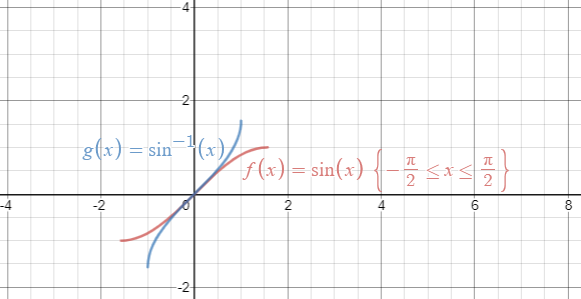
\includegraphics[width=9.5cm]{Q9_1.png}}
    \caption{Sine inverse and sine}
    \end{figure} 
\end{minipage}
\begin{minipage}{.5\textwidth}
    \begin{figure}[H]
    \centering{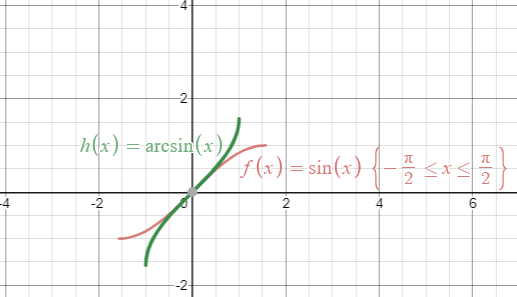
\includegraphics[width=9cm]{Q9_2.png}}
    \caption{Arcsine and sine}
    \end{figure} 
\end{minipage}\\
\begin{center}
\textbf{Characteristics of an arcsine function}\\
\end{center}
\begin{itemize}
    \item \textbf{Domain:} $x \in [-1, 1]$
    
    \item \textbf{Range:} $y \in \bigg[\dfrac{-\pi}{2},\dfrac{\pi}{2}\bigg]$
    
    \item \textbf{x-intercept(s):} $(0,0)$
    
    \item \textbf{y-intercept(s):} $(0,0)$
    
    \item \textbf{Interval of increase:} $[-1,1]$
    
    \item \textbf{Interval of decrease:} No interval of decrease
    
    \item \textbf{Injective and/or surjective:} Injective
    
    \item \textbf{Discontinuities:} There does not exist a value for $y$ if $x > \dfrac{\pi}{2}$ or $x < - \dfrac{\pi}{2}$
    
    \item \textbf{Symmetry:} Odd function. $f(x) = -f(-x)$
    
    \item \textbf{End behaviours:} No end behaviours
\end{itemize}

\newpage

%% PROBLEM 10
\item Consider the series $$\sum\limits_{i=1}^{n} i\left(\left(\dfrac{1+(-1)^{i+1}}{2}\right)\sin(x) + \left(\dfrac{1-(-1)^{i+1}}{2}\right)\cos(x)\right)$$

\begin{enumerate}
\item Determine $S_7$, the seventh partial sum of the series. \\

\textbf{Solution:}\\
Investigate a pattern by determining the first three terms. Sub in $i = 1$, $i = 2$, $i = 3$.\\
Sub in $i = 1$
\begin{align*}
    t_1 &= i \left(\left(\dfrac{1+(-1)^{i+1}}{2}\right)\sin(x) + \left(\dfrac{1-(-1)^{i+1}}{2}\right)\cos(x)\right) \\
    t_1 &= 1 \left(\left(\dfrac{1+(-1)^{1+1}}{2}\right)\sin(x) + \left(\dfrac{1-(-1)^{1+1}}{2}\right)\cos(x)\right)\\
    t_1 &= \left(\dfrac{1+(-1)^{2}}{2}\right)\sin(x) + \left(\dfrac{1-(-1)^{2}}{2}\right)\cos(x) \\
    t_1 &= \left(\dfrac{1+1}{2}\right)\sin(x) + \left(\dfrac{1-1}{2}\right)\cos(x) \\
    t_1 &= \left(\dfrac{2}{2}\right)\sin(x) + \left(\dfrac{0}{2}\right)\cos(x) \\
    t_1 &= \sin(x)
\end{align*}
Sub in $i = 2$
\begin{align*}
    t_2 &= i \left(\dfrac{1+(-1)^{i+1}}{2}\right)\sin(x) + \left(\dfrac{1-(-1)^{i+1}}{2}\right)\cos(x) \\
    t_2 &= 2 \left(\left(\dfrac{1+(-1)^{2+1}}{2}\right)\sin(x) + \left(\dfrac{1-(-1)^{2+1}}{2}\right)\cos(x)\right)\\
    t_2 &= 2 \left(\left(\dfrac{1+(-1)^{3}}{2}\right)\sin(x) + \left(\dfrac{1-(-1)^{3}}{2}\right)\cos(x)\right) \\
    t_2 &= 2 \left(\left(\dfrac{1-1}{2}\right)\sin(x) + \left(\dfrac{1+1}{2}\right)\cos(x)\right) \\
    t_2 &= 2 \left(\left(\dfrac{0}{2}\right)\sin(x) + \left(\dfrac{2}{2}\right)\cos(x) \right)\\
    t_2 &= 2\cos(x) 
\end{align*}
Sub in $i = 3$
\begin{align*}
    t_3 &= i \left(\left(\dfrac{1+(-1)^{i+1}}{2}\right)\sin(x) + \left(\dfrac{1-(-1)^{i+1}}{2}\right)\cos(x)\right) \\
    t_3 &= 3 \left(\left(\dfrac{1+(-1)^{3+1}}{2}\right)\sin(x) + \left(\dfrac{1-(-1)^{3+1}}{2}\right)\cos(x)\right) \\
    t_3 &= 3 \left(\left(\dfrac{1+(-1)^{4}}{2}\right)\sin(x) + \left(\dfrac{1-(-1)^{4}}{2}\right)\cos(x) \right)\\
    t_3 &= 3 \left(\left(\dfrac{1+1}{2}\right)\sin(x) + \left(\dfrac{1-1}{2}\right)\cos(x)\right) \\
    t_3 &= 3 \left(\left(\dfrac{2}{2}\right)\sin(x) + \left(\dfrac{0}{2}\right)\cos(x)\right) \\
    t_3 &= 3\sin(x)
\end{align*}

We can see that if $x$ is an even integer, the term $(-1)^{i+1}$ will be 1. Similarly, if $x$ is an odd integer, the term $(-1)^{i+1}$ will be -1. Moreover, the coefficient of $\sin(x)$ or $\cos(x)$ equals the term number, $n$. This means, when $i$ is odd, the element equals $i\sin(x)$, when $i$ is even, the element equals $i\cos(x)$. Knowing this, I can determine the seventh partial sum of the series much easier.\\
$$S_7 = \sin(x) + 2\cos(x) + 3\sin(x) + 4\cos(x) + 5\sin(x) + 6\cos(x) + 7\sin(x)$$
$$S_7 = 16\sin(x) + 12\cos(x)$$

\textbf{Therefore, $S_7 = 16\sin(x) + 12\cos(x)$}

%%================================    10 bbbbbbb    =================
\item Determine a closed form for the sum of the of the above series in the form $$\sum\limits_{i=1}^{n} i\left(\left(\dfrac{1+(-1)^{i+1}}{2}\right)\sin(x) + \left(\dfrac{1-(-1)^{i+1}}{2}\right)\cos(x)\right) = k \cdot \sin\left(x+\tan^{-1}\left(\frac{p}{q}\right)\right)$$
\end{enumerate}

\textbf{Solution:}\\
Recall from (a), when $i$ is even, the term is $i\sin(x)$, when $i$ is odd, the term is $i\cos(x)$. When added up into a series, it will be in the following form.
$$a\sin(x) + b\cos(x)$$
Since $a$ and $b$ are sums of $i$ and $i$ is a positive integer, I can say that $a$ and $b$ are also positive integers. Since $a$ and $b$ are positive integers, I can say that $\sqrt{a^2 + b^2} \geq 1$. This will be referred to later in the solution. For now, let's return to the the form $a\sin(x) + b\cos(x)$. I will manipulate this form into the closed form $k \cdot \sin\left(x+\tan^{-1}\left(\frac{p}{q}\right)\right)$.
\setcounter{equation}{0}
\begin{align}
    &= a\sin(x)+b\cos(x)\\
    &= \dfrac{\sqrt{a^2 + b^2}}{\sqrt{a^2 + b^2}}a\sin(x)+\dfrac{\sqrt{a^2 + b^2}}{\sqrt{a^2 + b^2}}b\cos(x) \xleftarrow[]{\textbf{multiplying by 1}}\\
    &= \sqrt{a^2 + b^2}\left(\dfrac{a\sin(x)}{\sqrt{a^2 + b^2}} + \dfrac{b\cos(x)}{\sqrt{a^2 + b^2}} \right) \xleftarrow[]{\textbf{factoring}}
\end{align}
Earlier, I said that $\sqrt{a^2 + b^2} \geq 1$. That means I am allowed to divide $a\sin(x)$ and $b\cos(x)$ by $\sqrt{a^2 + b^2}$ because I am not dividing by 0. Therefore, lines (2) and (3) above are valid.
Examine the coefficient of $a$ and $b$ in line (3).\\

1. Examine line (3), the coefficient of $\sin(x)$, $\dfrac{a}{\sqrt{a^2+b^2}}$. I can say that 
$\dfrac{a}{\sqrt{a^2}} = 1$, therefore $\dfrac{a}{\sqrt{a^2+b^2}} \leq 1$. Since $\dfrac{a}{\sqrt{a^2+b^2}}$ also consisted of positive integers only, I can say that $\dfrac{a}{\sqrt{a^2+b^2}} > 0$. Therefore, $$0 < \dfrac{a}{\sqrt{a^2+b^2}} \leq 1$$

2. Examine line (3), the coefficient of $\cos(x)$, $\dfrac{b}{\sqrt{a^2+b^2}}$. I can say that 
$\dfrac{b}{\sqrt{b^2}} = 1$, therefore $\dfrac{b}{\sqrt{a^2+b^2}} \leq 1$. Since $\dfrac{b}{\sqrt{a^2+b^2}}$ also consisted of positive integers only, I can say that $\dfrac{a}{\sqrt{a^2+b^2}} > 0$. But, since it is possible for $b$ to be 0 as $\cos(x)$ is 0 when $n = 1$, I can say that $\dfrac{a}{\sqrt{a^2+b^2}} \geq 0$. Therefore, $$0 \leq \dfrac{a}{\sqrt{a^2+b^2}} \leq 1$$\\

Because $0 < \dfrac{a}{\sqrt{a^2+b^2}} \leq 1$, it is within the range of cosine therefore I can say $\dfrac{a}{\sqrt{a^2+b^2}} = \cos(\theta)$.\\

Because $0 \leq \dfrac{a}{\sqrt{a^2+b^2}} \leq 1$, it is within the range of sine therefore I can say $\dfrac{b}{\sqrt{a^2+b^2}} = \sin(\theta)$.\\

There is another reason why I said $\dfrac{a}{\sqrt{a^2+b^2}} = \cos(\theta)$ and $\dfrac{b}{\sqrt{a^2+b^2}} = \sin(\theta)$. Consider a right triangle with sides $a$, $b$, and $c$, where $a$ and $b$ contain the right angled triangle and $c$ is the hypotenuse. Recall the Pythagorean theorem, I can say that $a^2 + b^2 = c^2$ or $\sqrt{a^2 + b^2} = c$. If angle $\theta$ is the angle in which I am calculating and $b$ is the opposite side, I can say that $\sin \theta = \dfrac{b}{c}$ and since $c = \sqrt{a^2 + b^2}$, $\sin \theta = \dfrac{b}{\sqrt{a^2+b^2}}$. That is the same case with $\cos \theta = \dfrac{a}{\sqrt{a^2+b^2}}$.

With these two things in mind, I can continue my manipulation from line (3) above.
\begin{align}
    &= \sqrt{a^2 + b^2}\left(\dfrac{a\sin(x)}{\sqrt{a^2 + b^2}} + \dfrac{b\cos(x)}{\sqrt{a^2 + b^2}} \right) \xleftarrow[]{\textbf{sub in $\cos(\theta)$ and $\sin(theta)$}} \\
    &= \sqrt{a^2 + b^2}\left(\cos(\theta)\sin(x) + \sin(\theta)\cos(x) \right)
\end{align}
Recall the addition and subtraction identity $\sin(A+B) = \sin(A)\cos(B) + \cos(A)\sin(B)$, I can rewrite $(\cos(\theta)\sin(x) + \sin(\theta)\cos(x))$ as $\sin(x + \theta)$.
\begin{align}
    &= \sqrt{a^2 + b^2}\left(\cos(\theta)\sin(x) + \sin(\theta)\cos(x) \right)\\
    &= \sqrt{a^2 + b^2} \times \sin(x+\theta) \xleftarrow[]{\textbf{addition identity}}
\end{align}
Recall the trigonometric identity $\tan \theta = \dfrac{\sin \theta}{\cos \theta}$, since $\sin = \dfrac{b}{\sqrt{a^2+b^2}}$ and $\cos = \dfrac{b}{\sqrt{a^2+b^2}}$, I can say that
$$\tan\theta = \dfrac{\sin\theta}{\cos\theta} = \dfrac{b}{\sqrt{a^2+b^2}} \times \dfrac{\sqrt{a^2+b^2}}{a} = \dfrac{b}{a}$$
Therefore, $\theta = \tan^-1\left(\dfrac{b}{a}\right)$
Returning to my manipulation, I can sub in $\theta = \tan^-1\left(\dfrac{b}{a}\right)$.
\begin{align}
    &= \sqrt{a^2 + b^2} \times \sin(x+\theta)\\
    &= \sqrt{a^2 + b^2} \times \sin(x+\tan^-1\left(\dfrac{b}{a}\right)) \xleftarrow[]{\textbf{sub in $\theta = \tan^-1\left(\dfrac{b}{a}\right)$}}
\end{align}
I can also let $\sqrt{a^2 + b^2}$ be $k$. Finally, I have
\begin{align}
    &= \sqrt{a^2 + b^2} \times \sin(x+\theta)\\
    &= k \times \sin \left(x+\tan^-1\left(\dfrac{b}{a}\right)\right)
\end{align}
\textbf{Therefore, line (11) is in the form $$\sum\limits_{i=1}^{n} i\left(\left(\dfrac{1+(-1)^{i+1}}{2}\right)\sin(x) + \left(\dfrac{1-(-1)^{i+1}}{2}\right)\cos(x)\right) = k \cdot \sin\left(x+\tan^{-1}\left(\frac{p}{q}\right)\right)$$}

\newpage  %% =================== NEW PAGE ===========================
Now, we can see that this series has two cases. Either $n$ is odd or $n$ is even. Recall that this series is always written in the form $$a\sin(x) + b\sin(x)$$
\begingroup
\addtolength{\jot}{0.8em}
\begin{minipage}{.5\textwidth}
    \begin{align*}
    &\textbf{Case 1: $\mathbf{n}$ is odd}\\
        a &= \dfrac{(n+1)^2}{4} \\
        b &= \dfrac{(n+1)(n-1)}{4}
    \end{align*}      
    \end{minipage}
    \begin{minipage}{.5\textwidth}
    \begin{align*}
    &\textbf{Case 2: $\mathbf{n}$ is even}\\
        a &= \dfrac{n^2}{4} \\
        b &= \dfrac{n^2 +2n}{4}
    \end{align*}
\end{minipage}
\endgroup\\

\textbf{Explanation of case 1:}\\
If n is odd,\\
$S_n = (1+3+5+...+n)\sin(x) + (2+4+6+...+(n-1))\cos(x)$\\

Examine the coefficient of $\sin(x)$, $(1+3+5+...+n)$. That is essentially the sum of positive odd integers. From Quora (source cited in declarations), I know that the sum of odd integers $(1+3+5+...+n) = n^2$ where $n$ equals \textit{the number of terms}. Recall Gauss' arithmetic series of consecutive natural numbers formula $1+2+3+4+...+n = \dfrac{n(n+1)}{2}$, where $n$ is the \textit{value of the highest term}. I will combine the formula to determine odd integers, $n^2$ and Gauss' formula, $\dfrac{n(n+1)}{2}$, to create a new formula that determines the sum of odd integers in terms of the \textit{value of the highest term}.\\

Consider series with FIVE terms, $S_5 = 1 + 3 + 5 + 7 + 9$. Let's assume we don't know that there are 5 terms in this series. The value of the highest term is 9. We can determine the number of terms in that series from the value of the highest term, in this case, 9.\\
Let $m$ be the number of terms present.
$$m = \left(\dfrac{9+1}{2}\right)^2$$
$$m = 5$$
Now that we know there are 5 terms in this series, we can use the formula I found on Quora, $m^2$ to determine the sum of the series.
Sub in $m = 5$
$$S_5 = m^2$$
$$S_5 = 5^2$$
$$S_5 = 25$$
Basically, the number 9, the highest value in the series is some number $z$, the number of terms in the series is some number $n$, and the nth partial sum of the series is $S_n = n^2$. I can deduce that
$$S_n = n^2$$
$$S_n = \left(\dfrac{m+1}{2}\right)^2$$
That is how I determine the coefficient of $\sin(x)$ when $n$ is odd. For the rest of the coefficients of $\sin(x)$ and $\cos(x)$, I also determined them in a similar way by working with one formula that determines the partial sum from TERM NUMBERS and another formula that determines the partial sum from the VALUE OF THE HIGHEST TERM.
Since $m$ is the number of terms and the number of terms squared equals the sum of the odd integers, I can say that $m^2$.\\

\textbf{Therefore:}\\
\textbf{if n is odd,} $$\mathbf{S_n = \dfrac{(n+1)^2}{4}\sin(x) + \dfrac{(n+1)(n-1)}{4}}\cos$$
\textbf{if n is even,} $$\mathbf{S_n = \dfrac{n^2}{4}\sin(x) + \dfrac{n^2 +2n}{4}\cos(x)}$$







\newpage


\end{enumerate}
\end{document} 
